%!TEX root = ../thesis.tex
% **************************** Define Graphics Path **************************
\ifpdf
\graphicspath{{Chapter4/Figs/Raster/}{Chapter4/Figs/PDF/}{Chapter4/Figs/}}
\else
\graphicspath{{Chapter4/Figs/Vector/}{Chapter4/Figs/}}
\fi


%*******************************************************************************
%****************************** Fourth Chapter *********************************
%*******************************************************************************


\chapter{Machine Learning}
\label{chapter4}
The field of Machine learning has been going through a renaissance in the past decade, mainly due to the spark ignited by an increase in computational power and the advent of deep learning~\cite{goodfellow2016deep}. In this chapter we present only the bare necessities needed to understand the methodology presented in the following chapter. We introduce basic concepts, the multilayer perceptron, convolutional layers, and discuss the role symmetry plays in designing neural networks for a task and why it is important in applications to lattice models.  

\section{Fundamentals}

\section{Neural Networks}
\begin{figure}[h]
	\centering
	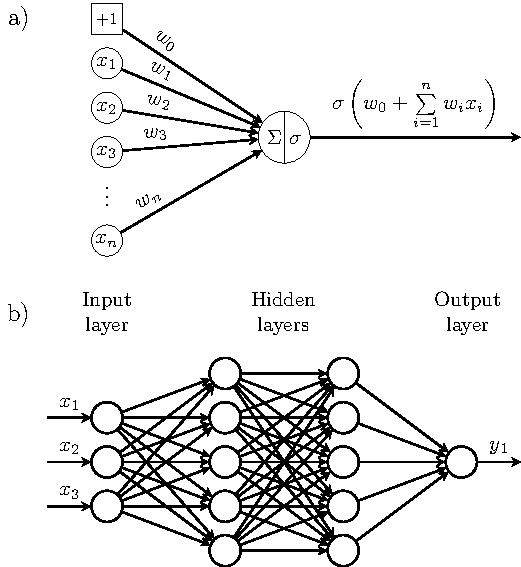
\includegraphics[width=0.7\linewidth]{Chapter4/Figs/Vector/mlp.pdf}
	\caption[Multilayer Perceptron]{\textbf{Multilayer Perceptron.}}
	\label{fig:mlp}
\end{figure}

\begin{figure}[h]
	\centering
	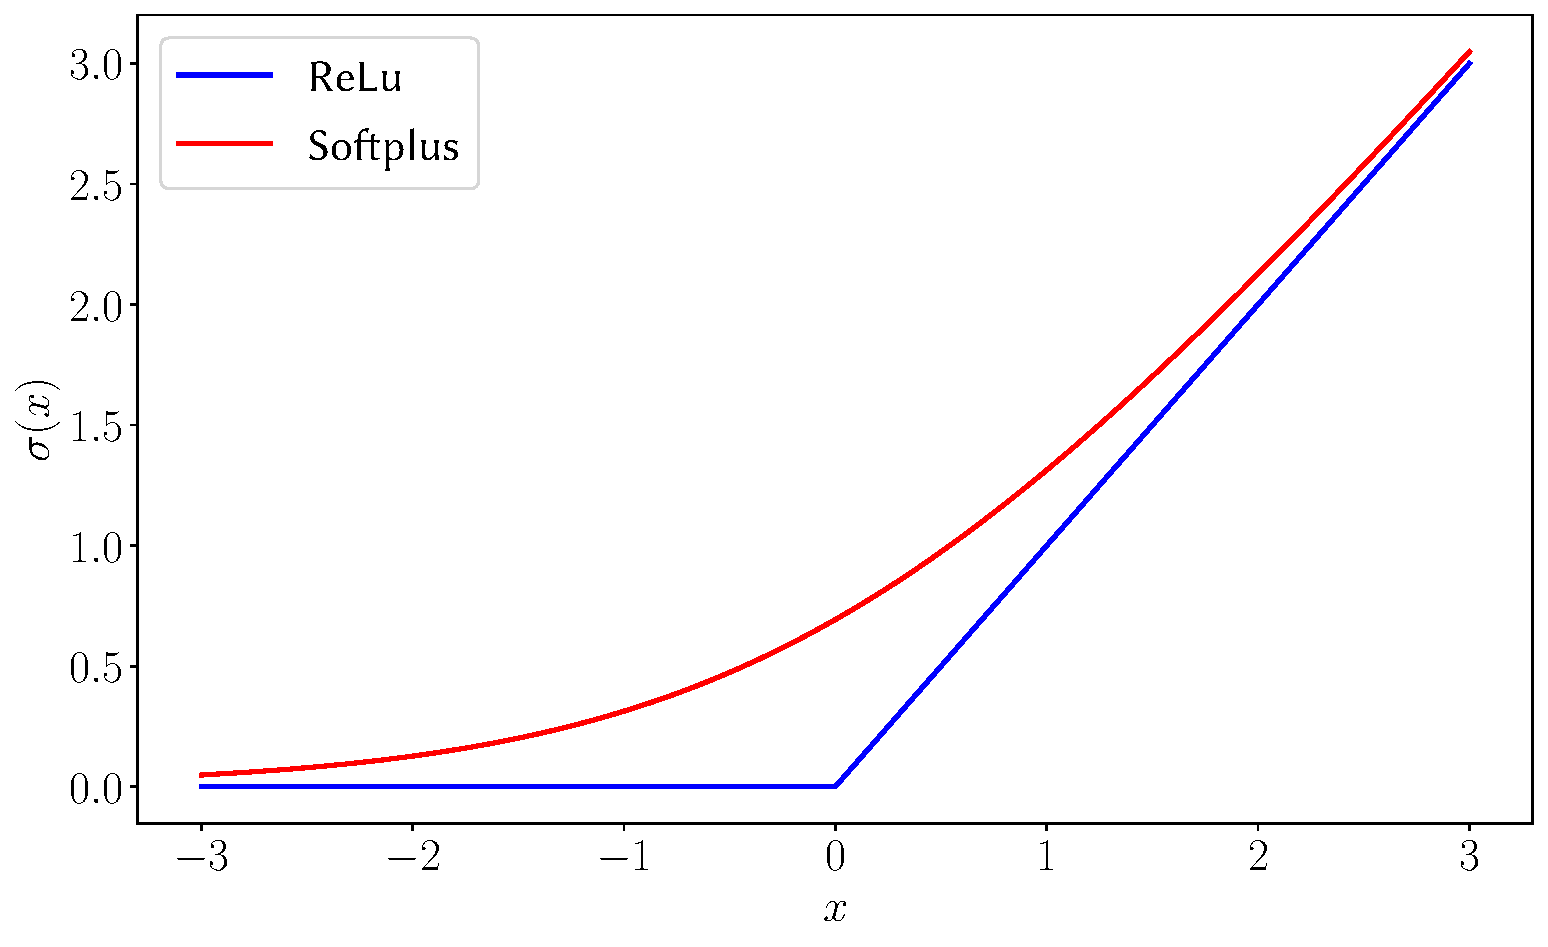
\includegraphics[width=0.7\linewidth]{Chapter4/Figs/Vector/activations}
	\caption[Activation functions]{\textbf{Activation functions.}}
	\label{fig:activations}
\end{figure}

\subsection{Convolutional Neural Networks}
\label{subsec:nn-cnn}

\begin{figure}
	\centering
	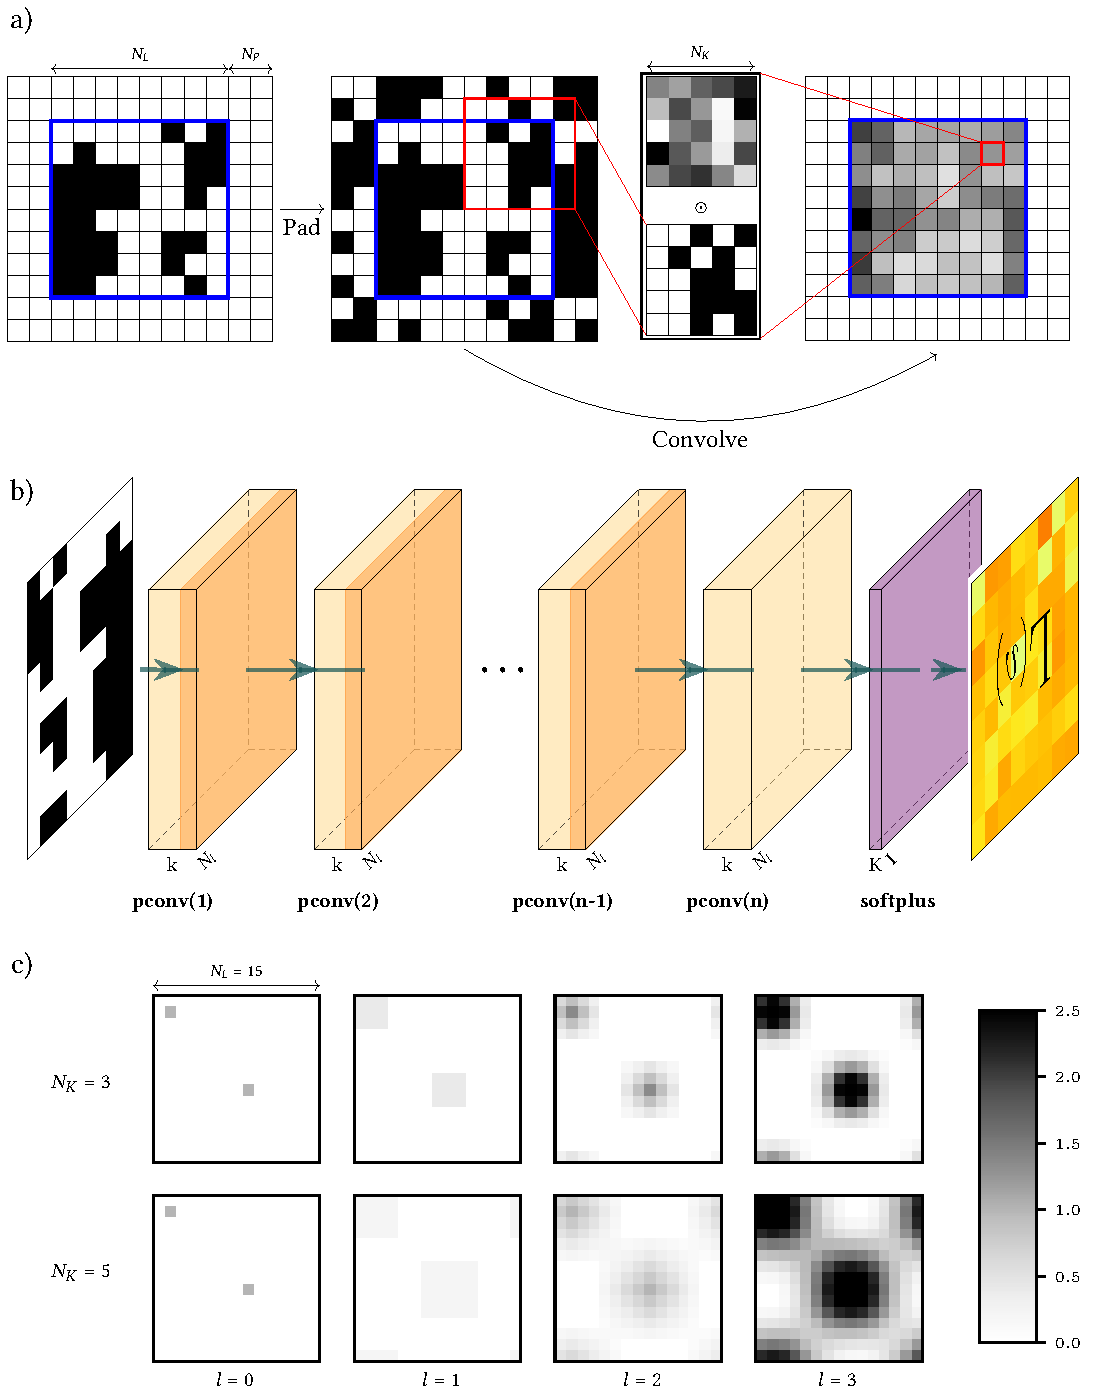
\includegraphics[width=\linewidth]{../diagrams/pcnn/pcnn}
	\caption[Periodic CNN]{\textbf{Periodic CNN}}
	\label{fig:pcnn}
\end{figure}


\subsection{Graph Neural Networks}
\label{subsec:nn-gnn}